\documentclass[tikz,border=5pt]{standalone}
\usepackage{tikz}
\usetikzlibrary{shapes.geometric,arrows.meta,positioning,calc,fit,backgrounds,shadows.blur,decorations.pathreplacing}
\usepackage{amsmath,amssymb}
\usepackage{helvet}
\renewcommand{\familydefault}{\sfdefault}

% Professional Color Palette (Nature / Elsevier Journal Quality)
\definecolor{themeBlue}{RGB}{24, 76, 120}
\definecolor{themeBlueLight}{RGB}{234, 242, 250}
\definecolor{themeBlueBorder}{RGB}{90, 140, 190}

\definecolor{themeTeal}{RGB}{18, 120, 120}
\definecolor{themeTealLight}{RGB}{230, 246, 246}
\definecolor{themeTealBorder}{RGB}{70, 170, 170}

\definecolor{themeAmber}{RGB}{180, 100, 20}
\definecolor{themeAmberLight}{RGB}{254, 246, 235}
\definecolor{themeAmberBorder}{RGB}{225, 160, 80}

\definecolor{themePurple}{RGB}{95, 45, 130}
\definecolor{themePurpleLight}{RGB}{245, 238, 250}
\definecolor{themePurpleBorder}{RGB}{160, 110, 195}

\definecolor{themeGreen}{RGB}{35, 125, 60}
\definecolor{themeGreenLight}{RGB}{235, 248, 238}
\definecolor{themeGreenBorder}{RGB}{100, 185, 125}

\definecolor{themeGray}{RGB}{70, 75, 85}
\definecolor{themeGrayLight}{RGB}{245, 246, 248}
\definecolor{themeGrayBorder}{RGB}{180, 185, 195}

\definecolor{alertRed}{RGB}{195, 40, 40}

\begin{document}
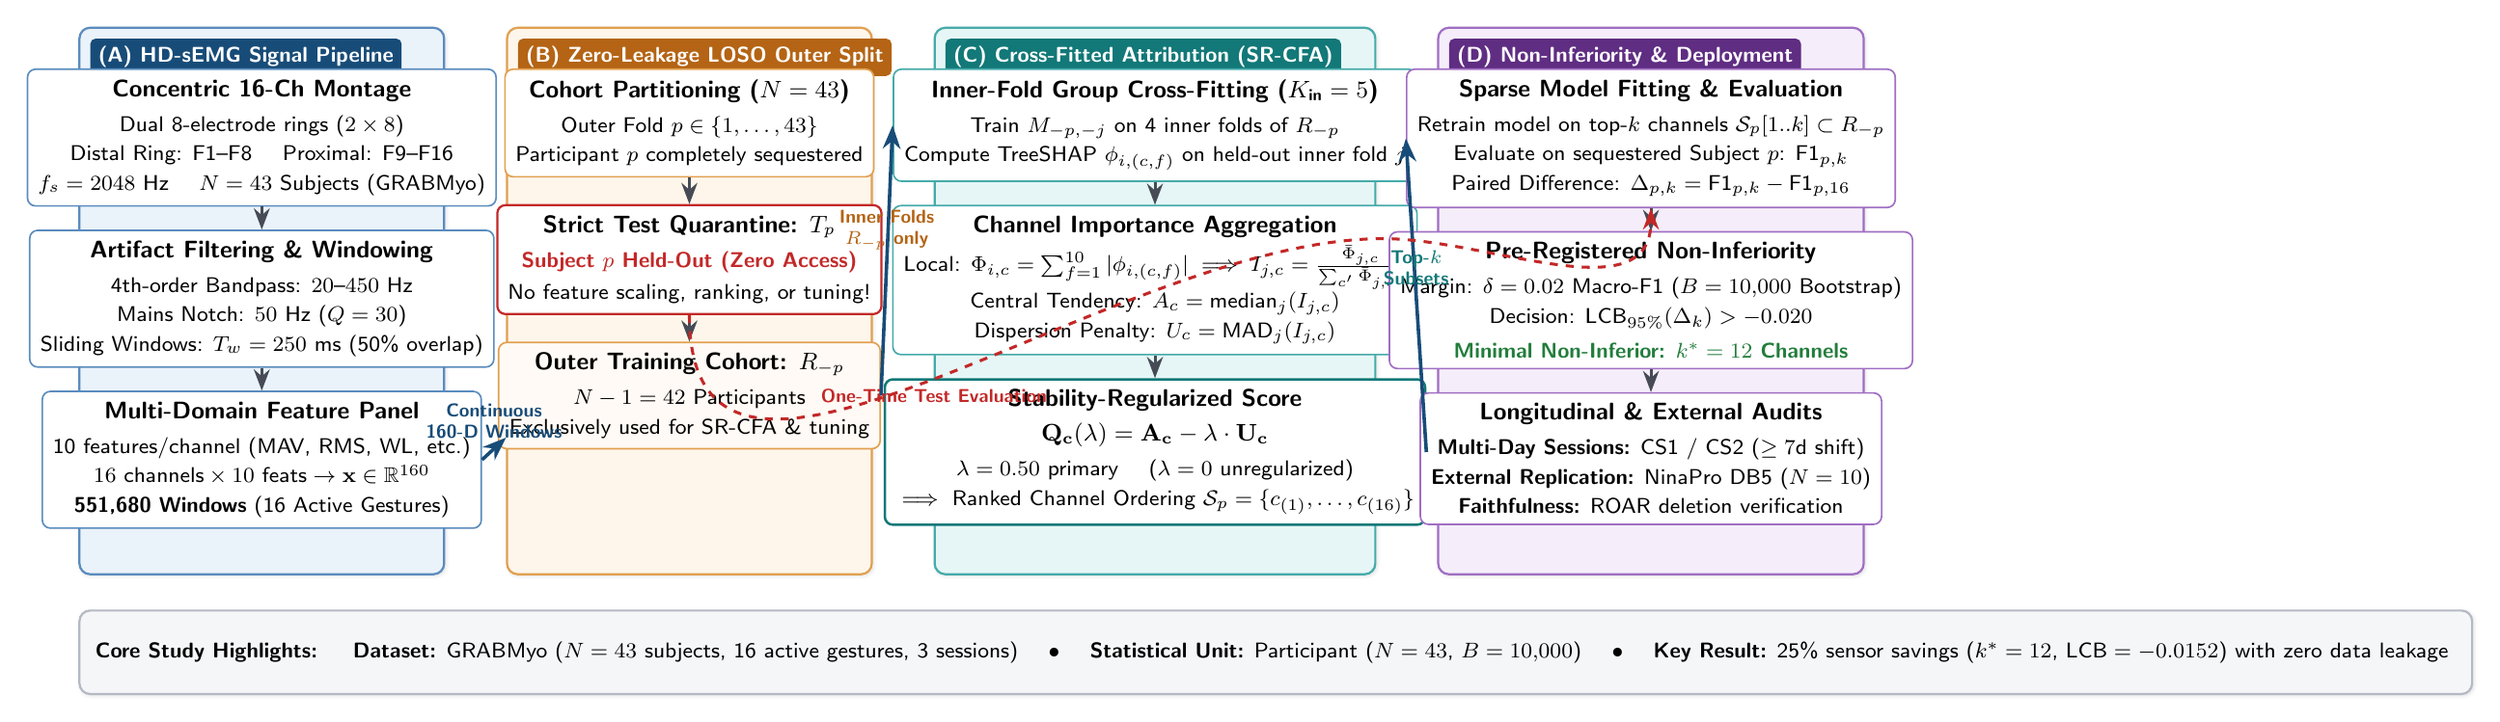
\begin{tikzpicture}[
    font=\small,
    >=Stealth,
    node distance=0.6cm and 0.8cm,
    every node/.style={align=center},
    card/.style={
        rounded corners=4pt,
        line width=0.8pt,
        inner sep=6pt,
        blur shadow={shadow blur steps=3, shadow blur radius=1.5pt, shadow opacity=15, shadow xshift=0.5pt, shadow yshift=-0.5pt}
    },
    header/.style={
        font=\bfseries\footnotesize,
        text=white,
        rounded corners=2pt,
        inner sep=3pt
    },
    subcard/.style={
        rounded corners=3pt,
        line width=0.6pt,
        inner sep=4pt,
        fill=white
    },
    flowline/.style={
        ->,
        line width=1.1pt,
        color=themeGray
    },
    accentline/.style={
        ->,
        line width=1.3pt,
        color=themeBlue
    }
]

% ==============================================================================
% SECTION A: HD-sEMG ACQUISITION & SIGNAL PROCESSING
% ==============================================================================
\node[card, fill=themeBlueLight, draw=themeBlueBorder, minimum width=4.8cm, minimum height=7.2cm] (secA) at (0, 0) {};
\node[header, fill=themeBlue, anchor=north west] at ($(secA.north west)+(0.15,-0.15)$) {(A) HD-sEMG Signal Pipeline};

% Sub-components in Section A
\node[subcard, draw=themeBlueBorder, minimum width=4.4cm, below=0.55cm of secA.north] (montage) {
    \textbf{Concentric 16-Ch Montage}\\[2pt]
    \footnotesize Dual 8-electrode rings ($2\times 8$)\\
    \footnotesize Distal Ring: F1--F8 \quad Proximal: F9--F16\\
    \footnotesize $f_s = 2048\text{ Hz}$ \quad $N=43$ Subjects (GRABMyo)
};

\node[subcard, draw=themeBlueBorder, minimum width=4.4cm, below=0.3cm of montage] (filtering) {
    \textbf{Artifact Filtering \& Windowing}\\[2pt]
    \footnotesize 4th-order Bandpass: $20\text{--}450\text{ Hz}$\\
    \footnotesize Mains Notch: $50\text{ Hz}$ ($Q=30$)\\
    \footnotesize Sliding Windows: $T_w = 250\text{ ms}$ (50\% overlap)
};

\node[subcard, draw=themeBlueBorder, minimum width=4.4cm, below=0.3cm of filtering] (features) {
    \textbf{Multi-Domain Feature Panel}\\[2pt]
    \footnotesize 10 features/channel (MAV, RMS, WL, etc.)\\
    \footnotesize $16\text{ channels} \times 10\text{ feats} \to \mathbf{x} \in \mathbb{R}^{160}$\\
    \footnotesize \textbf{551,680 Windows} (16 Active Gestures)
};

\draw[flowline] (montage) -- (filtering);
\draw[flowline] (filtering) -- (features);


% ==============================================================================
% SECTION B: STRICT ZERO-LEAKAGE LOSO PARTITIONING
% ==============================================================================
\node[card, fill=themeAmberLight, draw=themeAmberBorder, minimum width=4.8cm, minimum height=7.2cm, right=0.8cm of secA] (secB) {};
\node[header, fill=themeAmber, anchor=north west] at ($(secB.north west)+(0.15,-0.15)$) {(B) Zero-Leakage LOSO Outer Split};

\node[subcard, draw=themeAmberBorder, minimum width=4.4cm, below=0.55cm of secB.north] (losoSplit) {
    \textbf{Cohort Partitioning ($N=43$)}\\[2pt]
    \footnotesize Outer Fold $p \in \{1, \dots, 43\}$\\
    \footnotesize Participant $p$ completely sequestered
};

\node[subcard, draw=alertRed, fill=white, line width=0.8pt, minimum width=4.4cm, below=0.35cm of losoSplit] (testQuarantine) {
    \textbf{Strict Test Quarantine: $T_p$}\\[2pt]
    \footnotesize \textcolor{alertRed}{\textbf{Subject $p$ Held-Out (Zero Access)}}\\[1pt]
    \footnotesize No feature scaling, ranking, or tuning!
};

\node[subcard, draw=themeAmberBorder, fill=themeAmberLight!50, minimum width=4.4cm, below=0.35cm of testQuarantine] (trainCohort) {
    \textbf{Outer Training Cohort: $R_{-p}$}\\[2pt]
    \footnotesize $N-1 = 42$ Participants\\
    \footnotesize Exclusively used for SR-CFA \& tuning
};

\draw[flowline] (losoSplit) -- (testQuarantine);
\draw[flowline] (testQuarantine) -- (trainCohort);


% ==============================================================================
% SECTION C: STABILITY-REGULARIZED CROSS-FITTED ATTRIBUTION (SR-CFA)
% ==============================================================================
\node[card, fill=themeTealLight, draw=themeTealBorder, minimum width=5.8cm, minimum height=7.2cm, right=0.8cm of secB] (secC) {};
\node[header, fill=themeTeal, anchor=north west] at ($(secC.north west)+(0.15,-0.15)$) {(C) Cross-Fitted Attribution (SR-CFA)};

\node[subcard, draw=themeTealBorder, minimum width=5.4cm, below=0.55cm of secC.north] (innerCV) {
    \textbf{Inner-Fold Group Cross-Fitting ($K_{\text{in}}=5$)}\\[2pt]
    \footnotesize Train $M_{-p,-j}$ on 4 inner folds of $R_{-p}$\\
    \footnotesize Compute TreeSHAP $\phi_{i,(c,f)}$ on held-out inner fold $j$
};

\node[subcard, draw=themeTealBorder, minimum width=5.4cm, below=0.3cm of innerCV] (aggregation) {
    \textbf{Channel Importance Aggregation}\\[2pt]
    \footnotesize Local: $\Phi_{i,c} = \sum_{f=1}^{10} |\phi_{i,(c,f)}| \implies I_{j,c} = \frac{\bar{\Phi}_{j,c}}{\sum_{c'} \bar{\Phi}_{j,c'}}$\\
    \footnotesize Central Tendency: $A_c = \text{median}_j(I_{j,c})$\\
    \footnotesize Dispersion Penalty: $U_c = \text{MAD}_j(I_{j,c})$
};

\node[subcard, draw=themeTeal, line width=0.9pt, fill=white, minimum width=5.4cm, below=0.3cm of aggregation] (scoring) {
    \textbf{Stability-Regularized Score}\\[2pt]
    \small $\mathbf{Q_c(\lambda) = A_c - \lambda \cdot U_c}$\\[2pt]
    \footnotesize $\lambda=0.50$ primary \quad ($\lambda=0$ unregularized)\\
    \footnotesize $\implies$ Ranked Channel Ordering $\mathcal{S}_p = \{c_{(1)}, \dots, c_{(16)}\}$
};

\draw[flowline] (innerCV) -- (aggregation);
\draw[flowline] (aggregation) -- (scoring);


% ==============================================================================
% SECTION D: PRE-REGISTERED NON-INFERIORITY & VERIFICATION
% ==============================================================================
\node[card, fill=themePurpleLight, draw=themePurpleBorder, minimum width=5.6cm, minimum height=7.2cm, right=0.8cm of secC] (secD) {};
\node[header, fill=themePurple, anchor=north west] at ($(secD.north west)+(0.15,-0.15)$) {(D) Non-Inferiority \& Deployment};

\node[subcard, draw=themePurpleBorder, minimum width=5.2cm, below=0.55cm of secD.north] (sparseTrain) {
    \textbf{Sparse Model Fitting \& Evaluation}\\[2pt]
    \footnotesize Retrain model on top-$k$ channels $\mathcal{S}_p[1..k] \subset R_{-p}$\\
    \footnotesize Evaluate on sequestered Subject $p$: $\text{F1}_{p,k}$\\
    \footnotesize Paired Difference: $\Delta_{p,k} = \text{F1}_{p,k} - \text{F1}_{p,16}$
};

\node[subcard, draw=themePurpleBorder, minimum width=5.2cm, below=0.3cm of sparseTrain] (nonInfDecision) {
    \textbf{Pre-Registered Non-Inferiority}\\[2pt]
    \footnotesize Margin: $\delta = 0.02$ Macro-F1 ($B=10{,}000$ Bootstrap)\\
    \footnotesize Decision: $\text{LCB}_{95\%}(\Delta_k) > -0.020$\\[2pt]
    \footnotesize \textcolor{themeGreen}{\textbf{Minimal Non-Inferior: $k^* = 12$ Channels}}
};

\node[subcard, draw=themePurpleBorder, minimum width=5.2cm, below=0.3cm of nonInfDecision] (translation) {
    \textbf{Longitudinal \& External Audits}\\[2pt]
    \footnotesize \textbf{Multi-Day Sessions:} CS1 / CS2 ($\ge 7$d shift)\\
    \footnotesize \textbf{External Replication:} NinaPro DB5 ($N=10$)\\
    \footnotesize \textbf{Faithfulness:} ROAR deletion verification
};

\draw[flowline] (sparseTrain) -- (nonInfDecision);
\draw[flowline] (nonInfDecision) -- (translation);


% ==============================================================================
% INTER-SECTION FLOW CONNECTIONS
% ==============================================================================
\draw[accentline] (features.east) -- node[above, font=\scriptsize\bfseries, text=themeBlue, align=center]{Continuous\\160-D Windows} ($(secB.west)+(0, -1.8)$);

\draw[accentline] ($(trainCohort.east)+(0,0)$) -- node[above, font=\scriptsize\bfseries, text=themeAmber, align=center]{Inner Folds\\$R_{-p}$ only} ($(innerCV.west)+(0,0)$);

\draw[accentline] ($(scoring.east)+(0,0)$) -- node[above, font=\scriptsize\bfseries, text=themeTeal, align=center]{Top-$k$\\Subsets} ($(sparseTrain.west)+(0,0)$);

\draw[->, line width=1.1pt, dashed, color=alertRed] (testQuarantine.south) to[out=-90, in=180] node[below, font=\scriptsize\bfseries, text=alertRed]{One-Time Test Evaluation} ($(sparseTrain.south west)+(-0.3,-0.4)$) to[out=0, in=-90] (sparseTrain.south);

% ==============================================================================
% BOTTOM SUMMARY BANNER
% ==============================================================================
\node[card, fill=themeGrayLight, draw=themeGrayBorder, minimum width=23.4cm, minimum height=1.1cm, anchor=north west] at ($(secA.south west)+(0, -0.45)$) (banner) {
    \textbf{\footnotesize Core Study Highlights:} \quad
    \footnotesize \textbf{Dataset:} GRABMyo ($N=43$ subjects, 16 active gestures, 3 sessions) \quad $\bullet$ \quad
    \footnotesize \textbf{Statistical Unit:} Participant ($N=43$, $B=10{,}000$) \quad $\bullet$ \quad
    \footnotesize \textbf{Key Result:} 25\% sensor savings ($k^*=12$, $\text{LCB}=-0.0152$) with zero data leakage
};

\end{tikzpicture}
\end{document}
